\section{Product Development}\label{sec:product_development}
\subsection{Planing phase}
Before building the program, we brainstormed and created a Minimal Viable Product (MVP).
This MVP (which can be seen illustrate beneeth) is a general high level schematic outlining what our program is supposed to do.

\incfigure{figures/engMVP}{fig: MVP}{MVP}
Here we discussed what are the most essential parts, and came to the conclusion that the following things
were needed: The Users skills/abilities and the information from the vacant job position. These things
should be transformed into a custom application. 

After further consideration, we had encountered a problem, that generating a custom CV from nothing but
skills/abilities would create a very childlike, maybe even unreadable, application. This could be solved with a lot
of data, and therefore a lot of time calibrating the process of automatically creating sentences. This may also result
in a lower quality application, if this calibration doesn't happen. 
A CV, that might and might not even get through the "ATS/keyword scanner" outlined in the analysis. 

We therefore sought to instead create a filter, where the high quality sentences would be somewhat guaranteed and maintained.
This filter is only supposed to filter out all the unneccessary parts of a longer quality CV, into an application that
is ready to be sent. In other words, we decided to instead concentrate on creating a tool that aids
in sending out applications, instead of a CV generation program.

We then changed the MVP schematic to the following:
\incfigure{figures/Program_process_diagram}{fig: MVP}{Revised MVP}
This program is supposed to take in the keywords/job application, some formel requirements for
the structure of the new CV, and the originally long CV. 

The long CV should contain as many pages as possible, of all abilities and skills one has.
It should also include prior work experience, and anything else relevant on a CV. 

In this way, the program chooses the most important sentences, work experience and skills to be included,
and from the structural requirements creates a new CV.

From here we decided to organize our MVP into a UML diagram, to make it more apparent
what the essential functions were supposed to do, and which functions that were essential:
\incfigure{figures/UML}{fig: UML}{UML 1.0}

\subsection{Read.c}
\subsection{Filter.c}
%Indsæt filter strukturen som billede

%talk about what this part should do

\subsubsection{Removing Personal Pronouns}
After receiving the "free text" part, from the read.c file, we need to remove any personal pronouns.
We do this, since personal pronouns are quite unnecessary, since they don't add any substance to the sentences.
This is important to do since recruiters, as we talked about in the background section, spend a fraction of a minute
to look through the application. 
Having more unnecessary words will just distract the recruiters from understanding why they should hire you.
As talked about in the background section, not using personal pronouns increases your
chances of getting an interview by 55 percent.
\\
To remove all personal pronouns before filtering the rest of the text, we made the following function:
\incfigure{figures/personal_pronoun}{fig: pp function}{Remove personal pronouns function}
\\
It's a pretty simple function. To start it reads a certain section. Then it removes all personal pronouns at the start of each sentence in that section.
It loops through it, until there is no longer any personal pronouns left.
\\
In order to identity which words are personal pronouns, we have hardcoded a list of personal pronouns\cite{english_personal_pronouns} (including some words that are also unneccessary), that will be 'case insensitive compared'.
Each time a word is identified as a personal pronoun, a loop swaps all the words 1 to the left in the array, where the last word in that array will then be freed.
\\
There are also some hardcoded punctuation symbols, to indicate what is defined as the "start of a sentence". 
\\
this results in the following:
\incfigure{figures/personal_pronoun_ex}{fig: pp example}{Removing Personal Pronouns example}

As we can see, the filtered result is much cleaner and easier to read, without losing any information.
There is only problem left with it. Since the words are just shifted 1 to the left in the array, the sentence no longer begins
with a capitalized letter. This will later be fixed in a function in format.c, where such things will be formatted.

\subsubsection{Word Matching}
Word matching is one of the most interesting and most fundamental functions. 
It is the function that allows for keyword matching to exist, so that the application
may get through the ATS/keyword scan. How it works is it checks if input word 1, matches with input of word 2.
Where input 1 is the unfiltered original application text and input 2 is the keywords for the job posting.
If it is a match, then one might have an idea, that this section where the matched keyword is included may be important.
It does this using the function strcmp(n,r), which returns 0 if the string (or in our case, word) is identical.
\\
One quickly stumbles upon the following problems trying to match keywords.
\begin{itemize}
  \item 1. Since letters are ASCII defined, when comparing "Bathtime" with "bathtime", it won't return it as a match, even though it clearly is.
  \item 2. What if the word is the last word in a sentence? Comparing "Bathtime." with "Bathtime" should return a match, but it won't.
  \item 3. What if one has made simple spelling mistakes, such as spelling "Twillight" with 1 'l' instead of the required 2 'l's.
\end{itemize}

In order to overcome the first problem, one could easily make a loop, to loop through each letter, and check for both the capitalized and the small letters,
and return a match. This is especially easy, since the small letters always has a 32 higher ASCII value from their capitalized counterpart.
But after reading through the string library we found a function that does just the same comparison while ignoring capitalized letters: strcasecmp(n,r).
\\
The second problem has a quite a simple solution as well. Using the ASCII value of different kinds of punctuation symbols, we can easily remove these symbols by inserting a '\\0'. 
instead, thus making the string shorter.
\\
The third problem, is the trickiest one of the bunch. To solve this we decided on using the levenshtein algorithm. 
We found a translation of this algorithm in C and imported it\cite{levenshtein}.
The way this algorithm works, is by finding the distance between words. The larger the distance, the greater the difference between the words.
The algorithm determine distance as the amount of operations needed to change string A to string B. The algorithm uses 3 different types of operations:
\begin{itemize}
  \item 1. Insertion
  \item 2. Deletion
  \item 3. Substitution
\end{itemize}

to give an example of how these 3 operations can be applied:
\begin{itemize}
  \item Cat  Fat  (Substitution, 'C' with 'F')
  \item Fart  Far  (Deletion, removing the 'T')
  \item Sittin  Sitting  (Insertion, adding a 'G')
\end{itemize}

as an example, the levenshtein distance between "computer" and "cmptr" is 3.

This quickly raises a problem though, since the distance between cat and hat is smaller than the distance
between artificial and artificially. 
It's obvious that this isn't a spelling mistake, but 2 distinct words. Therefore we ran
some tests, to see how long words need to be, before something like this doesn't happen. 
The problem quickly becomes, that the longer the requirement the better the accuracy. 
But also the fewer words we can use the algorithm on, making the algorithm redundant.
We came to the conclusion based on our tests, that having words with greater than 4 letters, would be
the best compromise between length and accuracy.
\\
Now the problem is, what distance is accepted as 2 words being the same?
Here the problem also becomes, that grammatical endings are still the same words, just conjugated.
Based on a list of grammatical endings, the longest English ending adds a surfix of 3 letters\cite{grammar_endings}. Thus,
the max levenshtein distance should be under 4 letters.
Retesting using these values, we find that in nearly all arbitrary cases, the levenshtein algorithm matches the right words.
One problem may arise from the fact, that words can have different meanings in different contexts. Unfortunately taking account for semantics is out of the scope of this program.
\\
After using the levenshtein algorithm, one could argue that the remove punctuation function is redundant. But this is not the case. To the contrary, removing any
unnecessary parts of a string before using the levenshtein algorithm, makes the algorithm more precise. This is the case, since we can make sure the allowed distance
is smaller than what it had to be, if we hadn't removed punctuation.
\\
The overall structure of this functions ends up looking like the following:
\incfigure{figures/is_word_match}{fig: Is word match}{Word Matching}

The overall structure can be described as this:
\begin{figure}[h]
  \centering
  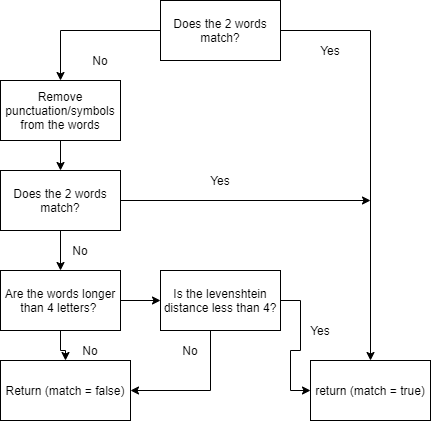
\includegraphics[height=3cm]{figures/is_match}
  \caption{Flow diagram of word matching}\label{fig:ie}
\end{figure}

The structure is constructed as a chain of if statements, to avoid unneccessary
calculations, so that the run time is optimized as much as possible.
\subsubsection{Section Density}
\incfigure{figures/section_density}{fig: density function}{Density and weight function}
Section density is based on the same concepts as in physics: Weight(mass)/Volume = Density.
In this case, weight is how many times in a section different words match with a keyword, and volume is how many words there
are in a section. The boundaries for the density function is as follows: Density goes from zero to one. 
Where zero is that there is no matches in a section, and one, is that every single word matches. Though a problem quickly arises
from doing it this way: A word may match with multiple keywords.
\begin{itemize}
  \item Section: "Great physic", keywords: "Physics, physicial".
\end{itemize}
Since the levenshtein distance is only 3 between physic and physical, and 1 between physic and physics,
the word physic will match with them both, thus potentilly creating a section with a density higher than the allowed 1.
To fix this issue, there was made a break condition for the weight loop, if a word from the section matched with a keyword.
The break function makes it such that no word could match with more than 1 keyword.
\\
Once the sections density has been calculated, the calculated density will be saved chonologically in a calloc'ed array of double values. 
This will be used to asses which sections are the most "important", from the definition that the more keyword matches, the greater the importance.
\\
Printing the result from this, we can see:
\incfigure{figures/density_example}{fig: density example}{Density array printet}
Thus it can easily be seen, which sections may be best suited for the job opening. 
In this case, an example of a job opening specializing in software.

To demonstrate that the functions work, it can be seen that both line 8 abd 9 gets printet with a result of exactly 1.
Even though one of the words match with 2, and the other, though misspelled, also matches with 2.

\subsubsection{Included Sections and Generation}
\incfigure{figures/includefunction}{fig: inclusionfunction}{Inclusion Function}
The process of finding the included sections can be described in three steps:
\begin{itemize}
  \item 1. Create tuple struct holding the density value, and the section ID.
  \item 2. Q-Sort the struct after density value.
  \item 3. save what section ID's should be included in the final output, based on the density, in a bool array.
\end{itemize}
First a struct is created. This is to ensure, that after sorting after highest density, the origianl order is still maintained.
This is important, since it can make it unreadable, if all the sections are mumbo jumbo'ed around.
After that, a Q-sort algorithm is used from the standard library. This algorithm makes sure, that the highest density comes first.
\\
Next, a bool array is created and calloc'ed. The values for the bool array are determined following this flowchat:
\incfigure{figures/include_flow}{fig: inclusion flowchart}{Flow diagram of the bool array}
In order to determin what sections should be included, a while loop is run, until a certain amount of words are included.
The amount of allowed words in the output is restricted to around 650, as that is the range, which grants the most amount of interviews.
That is, according to the research as described in the background section.
\\ \\
Here is an example, of it working: 
\incfigure{figures/bool_example}{fig: bool diagram}{Example of the bool array} 

The generation of the cv is quite simple in theory. All it does, is include all sections that the bool array determins should be included, and saves it into a long string.
Starting from the lowest section ID to the highest ID. 
The process of getting here is a little more complex, since it requires a lot of dynamic arrays, and inserting a lot of Null terminators, such  that it doesn't print null pointers.
This part isn't that interesting, but if you're interested, you can see it here:
\incfigure{figures/generate}{fig: generate function}{Text Generation Function}

\subsection{Format.c}
After the CV has been filtered then our next plan is to print the text to a latex format, and afterwords compile it to a pdf 

\subsection{CV-Gen.c}
\subsection{Makefile}

\subsection{TKOP-model}
A good way to describe the production could be the TVOP-model also known as technique, knowledge, organization and product.
It gives an easy impression of what the project group had performed.
First the technique, and to create a product for our project is essential to find a solution, 
one must use a number of techniques including C-programming, latex and github techniques.
Those techniques is good way to establish and find our solution. C-programming can help us to produce a CV using the techniques
of commands, functions etc. Latex is a good method to have a fine structured format, 
also it will help the writer and reader to read in the future. \newline

This takes one to have a fair amount of knowledge about the functions.
First of all knowledge about a CV, and how to use the knowledge is a important factor.
We have researched programming online about the functions that we didn't know about, 
and afterwords we will implement this to our code and see if it's working. If not then we can research more about the exact problem.
That's the waterfall model we have been used, not directly but it has been done in order to our code works.
\incfigure{figures/vandfald}{fig: Waterfall}{Waterfall model}
It has the elements that has been implemented in our coding. First we have the requirements for the program, 
so we can have functionally program, next we will design with the help from a UML diagram, 
so we know what should have in the program. Implementation of the program comes next, so we could test it later, 
and if we have other suggestions for improvement then we can write it down for further development.

In the process of coding the product, we choose to use a vertical work distribution, as many of the product
components can be made parallel to each other. We have divided it to several functions, 
so all of the group members can either alone or in pairs to get them done.
Each small group still needs to know future updates about the development with the functions, so the program can be put together.
To get an overview, we have made temporary division of labor
schedule, so the group can clearly see what can be done at the same time.

At last there is a product, a program from C that wil 